%iso-8859-2 encoding
\chapwithtoc{Opengl-Android application, Knots animator} % (fold)
\label{cha:Opengl-Android application}
\url{http://code.google.com/p/opengl-android/}

\section*{Problem definition} % (fold)
\label{sec:Problem definition}
Climbers have to use knots a lot. It is difficult to learn them all
and it is even harder to explain it by words.

I experienced few times a situation when pair of climbers
were arguing how to bind a knot before belaying each other
30 meters above a ground.

It will be really handy to have not only a learning tool
how to bind all necessary knots, but also a reference, 
which can be understandable quickly to every one.
% section* Problem definition (end)

\section*{User stories} % (fold)
\label{sec:User stories}
\begin{itemize}
  \item As a user, I want to press a button and launch Knot animator. 
  \item As a user, I want in running Knot animator press options button and view settings.
  \item As a user, I want to choose knots via "Knot selections" in opened settings.
  \item As a user, I want to set up Knot animator as a screen saver by pressing button in opened settings.
%  \item As a user, I want to press the cancel button in order to see the last knot.
  \item As a user, I want to view knot in 3D after choosing the knot.
  \item As a user, I want to turn around the knot by touching the screen.
  \item As a user, I want to zoom the knot in and out.
  \item {\bf Starting application:} After start, a user will see a default knot in 3D as if he chose it manually.
  \item As a user, I want to set up the default knot on the screen launched from the opened settings.
  \item {\bf Launching animation:}  As a user, I want to just click the display knot in order to see the animation how the knot is binded.
  \item {\bf Pausing animation:} As a user, I want to click the display to stop the animation.
  \item {\bf Canceling the animation:} As a user, I want to press the cancel button in order to stop the animation and back display the knot.
  \item {\bf Exiting the application:} As a user, I have to see one of the knots and press cancel button. 
  \item {\bf Loading multiple knots:} As a user, I want to load set of models by specifying their path in Xml file and loading only the settings from Xml file.
\end{itemize}

% section User stories (end)

\section*{Solution and description of the project} % (fold)
\label{sec:Solution}
The aim of this application is to be an always ready advisor, which will
present even to a child how a knot can be bind. 

"Knots animator" should  allow users to display the set of knots from different angle
and furthermore the application should offer rendering of knots binding.

Different points of view together with colourisation of the knots bindings
allows user to more easily understand how one the knots are binded.
In order to achieve good quality of 3D rendering, "Knots animator" 
uses OpenGL ES and also a full screen mode. 
The option of running the application as a screen saver could be really interesting
for passionate climbers.

Last but not least the application loads knots definitions from a obj files,
which allows application easily deploy additional sets of knots to customers.
Moreover the users can define knot on their own, or whatever models they want.
In fact, Knot animator is Wavefront obj viewer with additional features.
% section* Solution (end)

\section*{Target users} % (fold)
\label{sec:Target users}
Target users can be found among climbers and outdoor lovers,
which likes nicely looking and simple to use applications.  
I suppose that especially climbing instructors will appreciate
to have additional learning tool and possibility 
of designing the models of knots themselves in Blender. 

Furthermore, anybody who can design any 3D model and exporting it in Wavefront obj
format, can use Knot Animator like 3D visualisation tool.
% section* Target users (end)

\section*{Technology used} % (fold)
\label{sec:Technology used}

\begin{itemize}
  \item Android - target platform 
  \item Android SDK - Java framework for Android
  \item Android NDK - Native framework for Android
  \item OpenGL ES 2.0 - graphical engine restricted to Android
  \item XML - definition language 
\end{itemize}

The Knot animator is an Android application, 
thats user interface was developed by using Android SDK framework.
Nevertheless the crucial part of knot rendering uses OpenGL ES 2.0,
which is a restricted OpenGL graphical engine for Android devices.

As we decided to render 3D graphics, the choice of OpenGL came naturally.
The OpenGL ES 2.0 engine provides both necessary functionality and due to
native implementation also a better performance.
OpenGL ES 2.0 does not support statical rendering pipeline, 
but only programmable pipeline. \footnote{OpenGL ES 1.0 support only statical pipeline}
As a consequence we have to implement our own vertex and fragment shaders.
It means that shades, lights, blending and lot more has to be implemented by a programmer.
On the other hand, we can adjust complexity of shaders according our needs.

In order to interface OpenGL from C++ we use JNI (Java Native Interface) wrapper.
You can learn more about why we do not access directly fro Java in Subsection ~\ref{problems}.

% section* Technology used (end)

\section*{Architecture} % (fold)
\label{sec:Architecture}
The Knot animator has simple application logic with clearly divided tasks.
\begin{itemize}
  \item First of all we store the knot definitions in XML files,
so the Knot animator has to able parse the definition XML file of every knot.
  \item Secondly in order to interact with user input and other applications the application 
  implements Activities \todo{ TodoActivity1}, \todo{TodoActivity2}.
  \item The crucial part of application is rendering the 3D animation. We use OpenGL ES 1.0,
      JNI in classes \todo{TODO viewerGL} \todo{JNI wrapper}.
\end{itemize}

\todon{ graph of classes}
\todon{application logic graph}


\section*{Features and Effort} % (fold)
\label{sec:Features and Effort}
Obviously the key feature is to render the knot in 3D using OpenGL ES.
However, OpenGL ES could be used in two different ways on Android platform.

The first possibility is to call OpenGL functions through Java wrapper.
Java wrapper allows programmers to avoid C/C++ programming of OpenGL.
On the other hand, problems with passing parameters, especially preallocated arrays,
force to use programmers to use workarounds.

The second attitude is to use JNI. JNI is also a Java wrapper around C/C++ but does not wrap the OpenGL,
but the whole application logic in class {\it Activity}. 
The possibility to handle application in C/C++ allows developers call OpenGL ES directly from C/C++.

We have chosen to use the second attitude and implement 3D rendering using OpenGL ES 2.0 and JNI.
The main reasons are:
\begin{itemize}
  \item Clear interface between OpenGL ES and Android application
  \item Big performance improvement
  \item My phone (Android 2.1 update) support OpenGL ES 2.0 only from C/C++.
  \item Scalability of OpenGL ES 2.0 rendering pipeline 
  \item Possibility of code reuse Linux/Windows OpenGL app in C++
  \item Learning JNI
\end{itemize}

However the crucial part of this application lies 
in choosing the right data representation for storing the shape of knots.
Most important qualities of the format are:
\begin{itemize}
    \item Easily create models in this formats
    \item Textual. As far as I am starting with 3D modeling, 
    I will need to debug it
    \item Understandable
    \item Support animation
\end{itemize}

At the end I choose Wavefront OBJ format. It does not support animation, but it turned out,
that I was experiencing a lot problems with simple rendering of 3D model,
so I skipped this feature. Otherwise, OBJ format has all mentioned qualities.

Others features like full screen invocation or animation selection
I consider not application specific and I expect
to use classical techniques of Android programming.

The "nice to have" features like animation colourising 
or loading knots through specifying XML file are not crucial 
for making decision about architecture of this application. 
I also expect, that their implementation will consume minor time
in meaning of the whole project.


\begin{tabular}{| l || c | c |  c | c |}
\hline
Feature & Priority & Implemented & Est. hours & Real hours\\
\hline
\hline
\textbf{Learning JNI} & high & YES &                 4 & 51.5\\
\textbf{Exploring ndk samples} & high & YES &       12 & 11.5\\
\textbf{OpenGL demo} & high & YES &                  4 & 25\\
\textbf{Running animation} & high & YES &           20 & 40\\
\textbf{Loading OBJ definition} & high & YES &       6 &  8.5\\
\textbf{Select model} & high & YES &                 1 & 10\\
\textbf{Full screen} & middle & YES &                3 &  0\\
\textbf{Screen saver} & middle & NO &                4 &  -\\
\textbf{Binding colourising} & middle & NO &         4 & -\\
\textbf{Viewpoint manual} change & low & YES &       2 & 5\\
\textbf{Docs \& refactoring} & middle & NO &         5 & 20\\
\textbf{Design of XML} & high & NO &                15 & 1\\
\hline
\textbf{Totally} & &                                80 & 172.5 \\
\hline
\end{tabular}
\begin{figure}
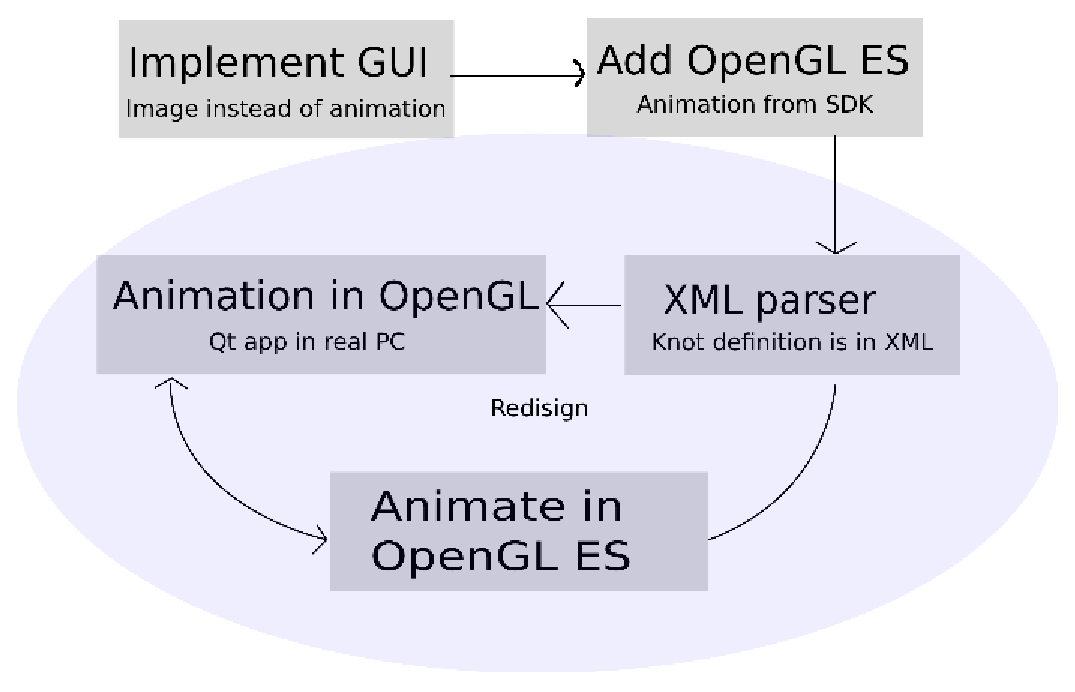
\includegraphics{work_flow.eps}
\label{work_flow}
\caption{Work flow}
\end{figure}

\todon{workflow of activities with dependecies}
\todon{ait/project/samples/hello-gl2        GL2JNIActivity  OpenGL 2.0   does not run on emulator}
% section* Features and Effort (end)

\section*{Technical problems} % (fold)
\label{sec:Technical problems}
I expect most problems in parsing the file with model definition
for storage of the 3D visualisation in OpenGL.

In fact, this assumption is was correct, because it was far to general.
I encountered problems in following implementation steps
\begin{itemize}
    \item Designing format for storing 3D representation of model. Finally, I decide to use some known 3D modeling format. Specifically Wavefront OBJ.
    \item Parse the OBJ file and load it for OpenGL
        \begin{itemize}
            \item I found out I, that Android does not support of accessing file system from C/C++ \footnote{It is possible to load some files through Android.mk like shared library. Access it via unzipping Apk and extract it. Obviously, it is very complicated, unsupported and statical approach.}
            \item I have to parse the OBJ file in Java first and then pass the data structures through {\bf JNI} to C/C++.
            As an unexperienced Java and Android programmer, using JNI was frustrating for me. 
            \item Transform the space effective structures passed to C++ into larger arrays, which are required by OpenGL
        \end{itemize}
    \item Debug the programmable pipeline
\end{itemize}

During testing the application and exploring the technologies I hit several problems.
Some of them I managed to solve, some of them results in giving up implementing some of the features.

For example, I found out that screen savers as such are totally unsupported in Android. Screen savers
used by vendors like HTC are implemented directly in custom build of Android, which is vendor dependent.
As I mentioned before, I choose Wavefront OBJ format, so I deliberately choose not to implement animations.

However, I coped with problems like bugs in library for parsing the OBJ file, which I used. 
I discovered them, repair and moved some parsing to the C++ part.
    
For a long time I had problem dividing the source code in C++ into several parts
and compile it using Android.mk (Android makefile). I made bad presumption and 
it really helped rereading the Android documentation after few month.

Another problem arose when I started programming the OpenGL pipeline.
GLSL(OpenGL Shading Language) is a standard, 
but I found out  only by googling
that Android implementation differs in tiny details (floats are 1.0 instead of 1.0f, etc).
Clearly, there is no possibility of debugging nor logging the GLSL on Android.

\subsection*{Tools and Hardware problems} % (fold)
The separation of the code allows me also to reuse the code and compile 
the C++ part like X11 Linux application. I used the X11 application for debugging
but only over Christmas, because my small notebook does not handle OpenGL 2.0 specification
needed by OpenGL ES 2.0 libraries.

It is worth to mention that current Android Emulator does not support OpenGL, 
I was forced to use my mobile all the time, 
but at the end I consider it an advantage.

Another serious problem of Java/C++ applications on Android 2.1 is a lack of support for C++ debugging.
For NDK8 is not possible to debug the C++ part, 
and even the building requires complicated setup.\footnote{Luckily, I found tutorial \href{http://mhandroid.wordpress.com/2011/01/23/using-eclipse-for-android-cc-development/}{Eclipse for C development} }
So the only debugging tool was LogCat, pen and paper.
% section* Technical problems (end)

\section*{Additional freatures} % (fold)
\label{sec:Additional freatures}
At first, all the features I had intended to implement and I did not are worth to implementing at first.
Another nice feature how to enrich this application is to implement
a voice advisor, who will give you spoken instruction during the animation.

% section* Additional freatures (end)
% chapter Opengl-Android application (end)
